%%%% Thanks to A. Gupta and R. Ravi for providing this template file.



\documentclass[11pt]{article}
\usepackage{amsfonts}
\usepackage{amssymb}
\usepackage{amstext}
\usepackage{amsmath}
\usepackage{xspace}
\usepackage{theorem}
\usepackage{color}
\usepackage[pdftex]{graphicx}
\usepackage{epsfig}
\usepackage[ruled,algosection,vlined,linesnumbered]{algorithm2e}
\usepackage{tikz}
\usepackage{float}
%\usepackage{layout}% if you want to see the layout parameters
                     % and now use \layout command in the body

% This is the stuff for normal spacing
\makeatletter
 \setlength{\textwidth}{6.5in}
 \setlength{\oddsidemargin}{0in}
 \setlength{\evensidemargin}{0in}
 \setlength{\topmargin}{0.25in}
 \setlength{\textheight}{8.25in}
 \setlength{\headheight}{0pt}
 \setlength{\headsep}{0pt}
 \setlength{\marginparwidth}{59pt}

 \setlength{\parindent}{0pt}
 \setlength{\parskip}{5pt plus 1pt}
 \setlength{\theorempreskipamount}{5pt plus 1pt}
 \setlength{\theorempostskipamount}{0pt}
 \setlength{\abovedisplayskip}{8pt plus 3pt minus 6pt}

 \renewcommand{\section}{\@startsection{section}{1}{0mm}%
                                   {2ex plus -1ex minus -.2ex}%
                                   {1.3ex plus .2ex}%
                                   {\normalfont\Large\bfseries}}%
 \renewcommand{\subsection}{\@startsection{subsection}{2}{0mm}%
                                     {1ex plus -1ex minus -.2ex}%
                                     {1ex plus .2ex}%
                                     {\normalfont\large\bfseries}}%
 \renewcommand{\subsubsection}{\@startsection{subsubsection}{3}{0mm}%
                                     {1ex plus -1ex minus -.2ex}%
                                     {1ex plus .2ex}%
                                     {\normalfont\normalsize\bfseries}}
 \renewcommand\paragraph{\@startsection{paragraph}{4}{0mm}%
                                    {1ex \@plus1ex \@minus.2ex}%
                                    {-1em}%
                                    {\normalfont\normalsize\bfseries}}
 \renewcommand\subparagraph{\@startsection{subparagraph}{5}{\parindent}%
                                       {2.0ex \@plus1ex \@minus .2ex}%
                                       {-1em}%
                                      {\normalfont\normalsize\bfseries}}
\makeatother

\newenvironment{proof}{{\bf Proof:  }}{\hfill\rule{2mm}{2mm}}
\newenvironment{proofof}[1]{{\bf Proof of #1:  }}{\hfill\rule{2mm}{2mm}}
\newenvironment{proofofnobox}[1]{{\bf#1:  }}{}\newenvironment{example}{{\bf Example:  }}{\hfill\rule{2mm}{2mm}}
\renewcommand{\thesection}{\lecnum.\arabic{section}}

\renewcommand{\theequation}{\thesection.\arabic{equation}}
\renewcommand{\thefigure}{\thesection.\arabic{figure}}

\newtheorem{fact}{Fact}[section]
\newtheorem{lemma}[fact]{Lemma}
\newtheorem{theorem}[fact]{Theorem}
\newtheorem{definition}[fact]{Definition}
\newtheorem{corollary}[fact]{Corollary}
\newtheorem{proposition}[fact]{Proposition}
\newtheorem{claim}[fact]{Claim}
\newtheorem{exercise}[fact]{Exercise}
\newtheorem{note}[fact]{Note}

% math notation
\newcommand{\R}{\ensuremath{\mathbb R}}
\newcommand{\Z}{\ensuremath{\mathbb Z}}
\newcommand{\N}{\ensuremath{\mathbb N}}
\newcommand{\F}{\ensuremath{\mathcal F}}

\newcommand{\size}[1]{\ensuremath{\left|#1\right|}}
\newcommand{\ceil}[1]{\ensuremath{\left\lceil#1\right\rceil}}
\newcommand{\floor}[1]{\ensuremath{\left\lfloor#1\right\rfloor}}




%%%%%%%%%%%%%%%%%%%%%%%%%%%%%%%%%%%%%%%%%%%%%%%%%%%%%%%%%%%%%%%%%%%%%%%%%%%
% Document begins here %%%%%%%%%%%%%%%%%%%%%%%%%%%%%%%%%%%%%%%%%%%%%%%%%%%%
%%%%%%%%%%%%%%%%%%%%%%%%%%%%%%%%%%%%%%%%%%%%%%%%%%%%%%%%%%%%%%%%%%%%%%%%%%%

\newcommand{\headings}[4]{
{\bf CO 759: Topics in Integer Programming} \hfill {{\bf Lecturer:} #1}\\
{{\bf Topic:} #2} \hfill {{\bf Date:} #3} \\
{{\bf Scribe:} #4}\\
\rule[0.1in]{\textwidth}{0.025in}
%\thispagestyle{empty}
}

\begin{document}
\headings{Ricardo Fukasawa}{Orbital Branching, Lattices and Basis Reduction}{Mar/3/2016}{William Justin Toth}
\newcommand{\lecnum}{0}

\section{Orbital Branching}

\paragraph{}
In this section we consider another technique for breaking symmetries while executing Branch and Bound called $\textit{orbital branching}$. As we will see it is very effective at breaking symmetries in some cases. It is even in use in commercial solvers like CPLEX.
\paragraph{}
The setting for this discussion is as follows. Let $P_I = \{x \in \{0,1\}^n : Ax \leq b \}$. Suppose we aim to minimize $c^Tx$ over $x \in P_I$. We will let $\tilde{G}$ denote the formulation group in this context. Suppose we are executing a Branch and Bound algorithm  which wants to branch on $x_j = 0$ or $x_j = 1$ are the root node of the Branch and Bound tree.
\paragraph{}
If we interpret our integer programming problem as modeling some combinatorial problem then fixing $x_j = 0$ is effectively just dropping corresponding object $j$ from solution. This does not gain much, particularly in the face of symmetry, where other variables may take on the role of $x_j$. That is to say, if $x_k \sim x_j$ then fixing $x_j = 0$ does not change much since we have equivalence.
\paragraph{}
Notice there is nothing in the general Branch and Bound procedure forcing us to choose the disjunction $x_j = 0$ or $x_j = 1$ for branching. Any disjunction will do. So let's choose one that better exploits the symmetry. Consider the disjunction
$$ \sum_{k \in orb(j, \tilde{G})} x_k \leq 0 \text{ or } \sum_{k \in orb(j, \tilde{G})} x_k \geq 1. $$
\begin{figure}[H]
\centering
\begin{tikzpicture}
\node[shape=circle, draw=black](A) at (0,0) {};
\node[shape=circle, draw=black](B) at (-1,-1){};
\node[shape=circle, draw=black](C) at (1,-1){};

\path[-] (A) edge node[left] { $\sum_{k \in orb(j, \tilde{G})} x_k \leq 0$}  (B);
\path[-] (A) edge node[right] { $\sum_{k \in orb(j, \tilde{G})} x_k \geq 1$}  (C);
\end{tikzpicture}
\caption{The Branch and Bound tree with disjunction under consideration}
\end{figure}
\begin{note} The condition $\sum_{k \in orb(j, \tilde{G})} x_k \leq 0$ is equivalent to saying $x_k = 0$ for all $k \in orb(j, \tilde{G})$.
\end{note}
\paragraph{}
Another way to interpret $\sum_{k \in orb(j, \tilde{G})} x_k \geq 1$ is to create one branch fixing each $x_k = 1$ for $k \in orb(j, \tilde{G})$. 
\begin{figure}[H]
\centering
\begin{tikzpicture}
\node[shape=circle, draw=black](A) at (0,1) {};
\node[shape=circle, draw=black](B) at (-1,-1){};
\node[shape=circle, draw=black](C) at (1,-1){};
\node[shape=circle, draw=black](D) at (5,-1){};
\path[-] (A) edge node[left] { $\sum_{k \in orb(j, \tilde{G})} x_k \leq 0$}  (B);
\path[-] (A) edge node[right] { $x_{k_1} = 1$}  (C);
\path[-] (A) edge node[right]{$x_{k_l} = 1$} (D);
\path[dashed](C) edge node[below]{$k_1, \dots, k_l$}(D);
\end{tikzpicture}
\caption{The Branch and Bound tree fixing each $x_k = 1$ for $k \in \{k_1, \dots, k_l\} = orb(j, \tilde{G})$}
\end{figure}
\paragraph{}
But this approach would potentially lead to many branches. Fortunately since
$$x_{k_1} \sim x_{k_2} \sim \dots \sim x_{k_l} $$
branching on each $x_{k_i}$ is equivalent, and we need only branch on $x_j$. Doing this is what is referred to as $\textit{orbital branching}$. Below is a figure visually representing the technique. We will follow with an example demonstrating the effectiveness of orbital branching.
\begin{figure}[H]
\centering
\begin{tikzpicture}
\node[shape=circle, draw=black](A) at (0,0) {};
\node[shape=circle, draw=black](B) at (-1,-1){};
\node[shape=circle, draw=black](C) at (1,-1){};

\path[-] (A) edge node[left] { $x_k = 0$ for all $k \in orb(j, \tilde{G})$}  (B);
\path[-] (A) edge node[right] {$x_j = 1$}  (C);
\end{tikzpicture}
\caption{The Branch and Bound tree with orbital branching at $x_j$}
\end{figure}
\subsection{Orbital Branching Example}
\paragraph{}
Consider the integer programming formulation of the maximum cardinality stable set problem (given a graph $G=(V,E)$ find a set of vertices with no edges between them as large as possible):
\begin{align*}
&\text{max} &\sum_{v\in V} x_v \\
&s.t. &x_j + x_j &\leq 1, &\text{for all $ij \in E$} \\
& &x_v &\in \{0,1\}, &\text{for all $v \in V$}.
\end{align*}
Suppose we are trying to solve the problem with input graph $G$ draw below:
\begin{figure}[H]
\centering
\begin{tikzpicture}
\node[shape=circle, draw=black](5) at (1,3) {5};
\node[shape=circle, draw=black](12) at (2,3) {12};
\node[shape=circle, draw=black](6) at (0,2) {6};
\node[shape=circle, draw=black](1) at (1,2) {1};
\node[shape=circle, draw=black](4) at (2,2) {4};
\node[shape=circle, draw=black](11) at (3,2) {11};
\node[shape=circle, draw=black](7) at (0,1) {7};
\node[shape=circle, draw=black](2) at (1,1) {2};
\node[shape=circle, draw=black](3) at (2,1) {3};
\node[shape=circle, draw=black](10) at (3,1) {10};
\node[shape=circle, draw=black](8) at (1,0) {8};
\node[shape=circle, draw=black](9) at (2,0) {9};

\path[-] (5) edge (6);
\path[-] (5) edge (1);
\path[-] (1) edge (6);

\path[-] (12) edge (4);
\path[-] (11) edge (4);
\path[-] (12) edge (11);

\path[-] (7) edge (2);
\path[-] (8) edge (2);
\path[-] (7) edge (8);

\path[-] (3) edge (10);
\path[-] (9) edge (10);
\path[-] (3) edge (9);

\path[-] (1) edge (2);
\path[-] (3) edge (2);
\path[-] (3) edge (4);
\path[-] (1) edge (4);
\end{tikzpicture}
\caption{Input graph $G$}
\end{figure}
If we solve the linear programming relaxation we obtain the solution $x_v = \frac{1}{2}$ for all $v \in V$. Let's say our algorithm decides to branch on $x_5$. The branch $x_5 = 1$ is used in both the original branching method and orbital branching. The graph for the subproblem with $x_5 = 1$ is shown below.
\begin{figure}[H]
\centering
\begin{tikzpicture}

\node[shape=circle, draw=black](12) at (2,3) {12};
\node[shape=circle, draw=black](4) at (2,2) {4};
\node[shape=circle, draw=black](11) at (3,2) {11};
\node[shape=circle, draw=black](7) at (0,1) {7};
\node[shape=circle, draw=black](2) at (1,1) {2};
\node[shape=circle, draw=black](3) at (2,1) {3};
\node[shape=circle, draw=black](10) at (3,1) {10};
\node[shape=circle, draw=black](8) at (1,0) {8};
\node[shape=circle, draw=black](9) at (2,0) {9};


\path[-] (12) edge (4);
\path[-] (11) edge (4);
\path[-] (12) edge (11);

\path[-] (7) edge (2);
\path[-] (8) edge (2);
\path[-] (7) edge (8);

\path[-] (3) edge (10);
\path[-] (9) edge (10);
\path[-] (3) edge (9);


\path[-] (3) edge (2);
\path[-] (3) edge (4);
\end{tikzpicture}
\caption{Subproblem for $x_5 = 1$}
\end{figure}
Now the other branch is where we see the difference. If the original branching strategy was used we would have the subproblem shown below.
\begin{figure}[H]
\centering
\begin{tikzpicture}
\node[shape=circle, draw=black](12) at (2,3) {12};
\node[shape=circle, draw=black](6) at (0,2) {6};
\node[shape=circle, draw=black](1) at (1,2) {1};
\node[shape=circle, draw=black](4) at (2,2) {4};
\node[shape=circle, draw=black](11) at (3,2) {11};
\node[shape=circle, draw=black](7) at (0,1) {7};
\node[shape=circle, draw=black](2) at (1,1) {2};
\node[shape=circle, draw=black](3) at (2,1) {3};
\node[shape=circle, draw=black](10) at (3,1) {10};
\node[shape=circle, draw=black](8) at (1,0) {8};
\node[shape=circle, draw=black](9) at (2,0) {9};

\path[-] (1) edge (6);

\path[-] (12) edge (4);
\path[-] (11) edge (4);
\path[-] (12) edge (11);

\path[-] (7) edge (2);
\path[-] (8) edge (2);
\path[-] (7) edge (8);

\path[-] (3) edge (10);
\path[-] (9) edge (10);
\path[-] (3) edge (9);

\path[-] (1) edge (2);
\path[-] (3) edge (2);
\path[-] (3) edge (4);
\path[-] (1) edge (4);
\end{tikzpicture}
\caption{Subproblem for original branching $x_5 = 0$}
\end{figure}
But if we use orbital branching we obtain the much smaller subproblem:
\begin{figure}[H]
\centering
\begin{tikzpicture}
\node[shape=circle, draw=black](1) at (1,2) {1};
\node[shape=circle, draw=black](4) at (2,2) {4};
\node[shape=circle, draw=black](2) at (1,1) {2};
\node[shape=circle, draw=black](3) at (2,1) {3};

\path[-] (1) edge (2);
\path[-] (3) edge (2);
\path[-] (3) edge (4);
\path[-] (1) edge (4);
\end{tikzpicture}
\caption{Subproblem for orbital branching $x_k = 0$ for all $k \in orb(5,\tilde{G})$}
\end{figure}
This shows the benefits obtained using an orbital branching strategy.
\section{Lattices and Basis Reduction}
\end{document}


